%-------------------------
%minimal-unix
%(c) H.Buchmann FHNW 2017
%export TEXINPUTS=.:${HOME}/fhnw/edu/:${HOME}/fhnw/edu/tinL/config/latex:${HOME}/fhnw/edu/config//:
%-------------------------
\documentclass{beamer}
\usepackage{latex/beamer}
%---------------------
%local defines
%(c) H.Buchmann FHNW 2009
%$Id$
%---------------------
\def \target {\raspberry\xspace}
\def \host {{\em Host \xspace}}


\usepackage[absolute]{textpos}
\setlength{\TPHorizModule}{1mm}
\setlength{\TPVertModule}{1mm}

\begin{document}

\newcommand{\md}{\cod{md-bbb-{\em version}.img}}
\newcommand{\mdev}{\cod{md-bbb-devel-{\em version}.tar.gz}}
\title[Minimal]{Ein kleines \unix}

\frame{\titlepage}

\begin{frame}{Ein kleines \unix}
 \begin{itemize}
  \item die einzelnen Komponenten
  \item für Test
  \item übersichtlich
  \item grosse Systeme haben ähnliche Komponenten
 \end{itemize}
\end{frame}

\begin{frame}{Die grossen Blöcke}{Übergänge}
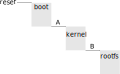
\includegraphics[width=\textwidth]{components.pdf}
\begin{textblock}{100}(10,50)
 \begin{description}[reset]
  \item[reset] start: BigBang
  \item[A] unprotected$\to$ protected ?
  \item[B] concurrency
 \end{description}
\end{textblock}
\end{frame}

\begin{frame}[fragile]{Boot:u-boot}{Zwei Files}
\begin{block}{reset}
{\tiny
\begin{verbatim}
U-Boot 2018.09 (Dec 18 2018 - 13:56:52 +0100)
\end{verbatim}
}
\end{block}
 \begin{itemize}
  \item \cod{MLO} Wegen TI
  \item \cod{u-boot.img}
 \end{itemize}
\begin{textblock}{100}(45,30)
 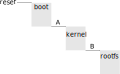
\includegraphics[width=0.75\textwidth]{components.pdf}
\end{textblock} 
\end{frame}

\begin{frame}[fragile]{Kernel}{Zwei Files}
\begin{block}{A}
{
\tiny
\begin{verbatim}
Booting Linux on physical CPU 0x0					       
Linux version 4.19.5 (buchmann@buchmannh) (gcc version 8.2.0 (GCC)) #6 SMP PRE8
\end{verbatim}
}
\end{block}
\begin{itemize}
 \item \cod{zImage} Der {\em kernel}
 \item \cod{am335x-boneblack-wireless.dtb} device tree
 \end{itemize}
\begin{textblock}{100}(45,30)
 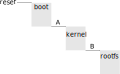
\includegraphics[width=0.75\textwidth]{components.pdf}
\end{textblock} 
\end{frame}

\begin{frame}[fragile]{RootFS: Viele Files}{Unser Interesse}
\begin{block}{B}
{
\tiny
\begin{verbatim}
VFS: Mounted root (ext4 filesystem) on device 179:2.
devtmpfs: mounted
Freeing unused kernel memory: 1024K

Please press Enter to activate this console. 
\end{verbatim}
}
\end{block}
\begin{itemize}
 \item \cod{linuxrc} Init-Process
 \item ...
\end{itemize}
\begin{textblock}{100}(45,25)
 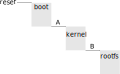
\includegraphics[width=0.75\textwidth]{components.pdf}
\end{textblock} 

\end{frame}

\begin{frame}{RootFS}{Flavours}
 \begin{itemize}
  \item nano
  \begin{itemize}
   \item Assembler ohne {\em libraries} \cod{s-nano.S}
   \item \c fast ohne {\em libraries} \cod{c-nano.c}
  \end{itemize}
  \item mini
  \begin{itemize}
   \item {\em libraries}
   \begin{itemize}
    \item static
    \item dynamic
   \end{itemize}
  \end{itemize}
  \item full
  \begin{itemize}
   \item \cod{busybox}
   \item \cod{ssh}
   \item ...
  \end{itemize}
 \end{itemize}
\end{frame}

\section{Nano}
\begin{frame}
\begin{center}
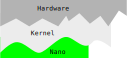
\includegraphics[width=0.75\textwidth]{nano.pdf}
\end{center}
\begin{itemize}
 \item \cod{config/Makefile}
 \item \cod{src/s-nano.S}
 \item \cod{src/c-nano.c}
\end{itemize}
\end{frame}

\section{Mini}
\begin{frame}
\begin{center}
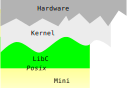
\includegraphics[width=0.5\textwidth]{mini.pdf}
\end{center}
\vspace{-5mm}
\begin{itemize}
 \item \cod{config/Makefile}
 \item \cod{src/mini.c}
 \begin{itemize}
  \item static
  \begin{description}
   \item[target-root] \cod{libc.a}
  \end{description}
  \item dynamic
  \begin{description}
   \item[target-root] \cod{libc.so}, \cod{loader}
  \end{description}
 \end{itemize}
\end{itemize}
\end{frame}

\subsection{Libraries}

\begin{frame}{Statische/Dynamische Bibliothek}{Kopie vs. Referenz}
 \begin{columns}
  \begin{column}{5cm}
   \begin{block}{Static}
   \begin{itemize}
    \item \hfill \vspace{-3mm}\fig{static.pdf}{0.5}{0}
    \item {\Large fr�hes} Binden
   \end{itemize}
   \end{block}
  \end{column}
  \begin{column}{5cm}
   \begin{block}{Dynamic}
    \begin{itemize}
    \item\hfill \vspace{-3mm}\fig{dynamic.pdf}{0.5}{0}
    \item {\Large sp�tes} Binden
    \end{itemize}
   \end{block}
  \end{column}
 \end{columns}
 \begin{block}{}
  \fig{legend.pdf}{0.5}{0}
 \end{block}
\end{frame}

\begin{frame}{Dynamische Bibliothek}{der Loader}
 \begin{itemize}
  \item \cod{/lib/ld-2.26.so}
 \end{itemize}
\end{frame}


%-------------------------
%exercises.tex
%(c) H.Buchmann FHNW 2019
%export TEXINPUTS=${HOME}/fhnw/edu/tinL/config/latex:${HOME}/fhnw/edu/config//:
%-------------------------
\documentclass{beamer}
\usepackage{latex/beamer}
%---------------------
%local defines
%(c) H.Buchmann FHNW 2009
%$Id$
%---------------------
\def \target {\raspberry\xspace}
\def \host {{\em Host \xspace}}

\begin{document}

\begin{frame}{18.Sept.2019}
\begin{itemize}
 \item Umgebung aufsetzen
 \begin{itemize}
  \item Linux
  \item git repo
 \end{itemize}
\item \target verbinden mit \host
 \begin{itemize}
  \item per USB
  \begin{itemize}
   \item serielle Schnittstelle 
   \item Internet
  \end{itemize}
  \item per WLAN
 \end{itemize}
\item sich auf dem \target zurechtfinden
\end{itemize}
\end{frame}

\begin{frame}{25.Sept.2019}
 \begin{itemize}
  \item Alles ist ein File
  \begin{itemize}
   \item \cod{sshfs} mount
   \item \cod{mount} SD-Karte
  \end{itemize}
  \item Netzwerk
  \begin{itemize}
   \item Host als Proxy
   \item Host als Gateway/Router
   \item \targetS via WiFi
  \end{itemize}
 \end{itemize}
\end{frame}

\begin{frame}{2.Okt. 2019}
 \begin{itemize}
  \item \targetS kleines Image auf SD-Karte
  \item Zugriff via serielle Schnittstelle
  \item via USB am lokalen Netz
  \begin{itemize}
    \item ssh \& sshfs
  \end{itemize}
  \item via Wi-Fi am Internet
 \end{itemize}
\end{frame}

\begin{frame}{9.Okt. 2019}
 \begin{itemize}
  \item init script für \targetS
  \item 5-kernel
  \begin{itemize}
   \item basic config
   \item USB Gadget
   \item WiFi \& firmware
  \end{itemize}
 \end{itemize}
\end{frame}

\begin{frame}{16.Okt. 2019}
 \begin{itemize}
  \item 6-crossdevelopment
  \begin{itemize}
   \item Programme in \cod{src} auf \host \& \targetS
   \item Vergleich Zeit von \cod{primes} auf \host \& \targetS
  \end{itemize}
 \end{itemize}
\end{frame}
\end{document}

\end{document}
